\documentclass[border=10pt]{standalone}

\usepackage{tikz}
\usepackage{tikzsymbols}
\usetikzlibrary{calc,patterns,shapes.geometric}

\def\centerarc[#1](#2)(#3:#4:#5){\draw[#1] ($(#2)+({#5*cos(#3)},{#5*sin(#3)})$) arc (#3:#4:#5);}

\begin{document}
	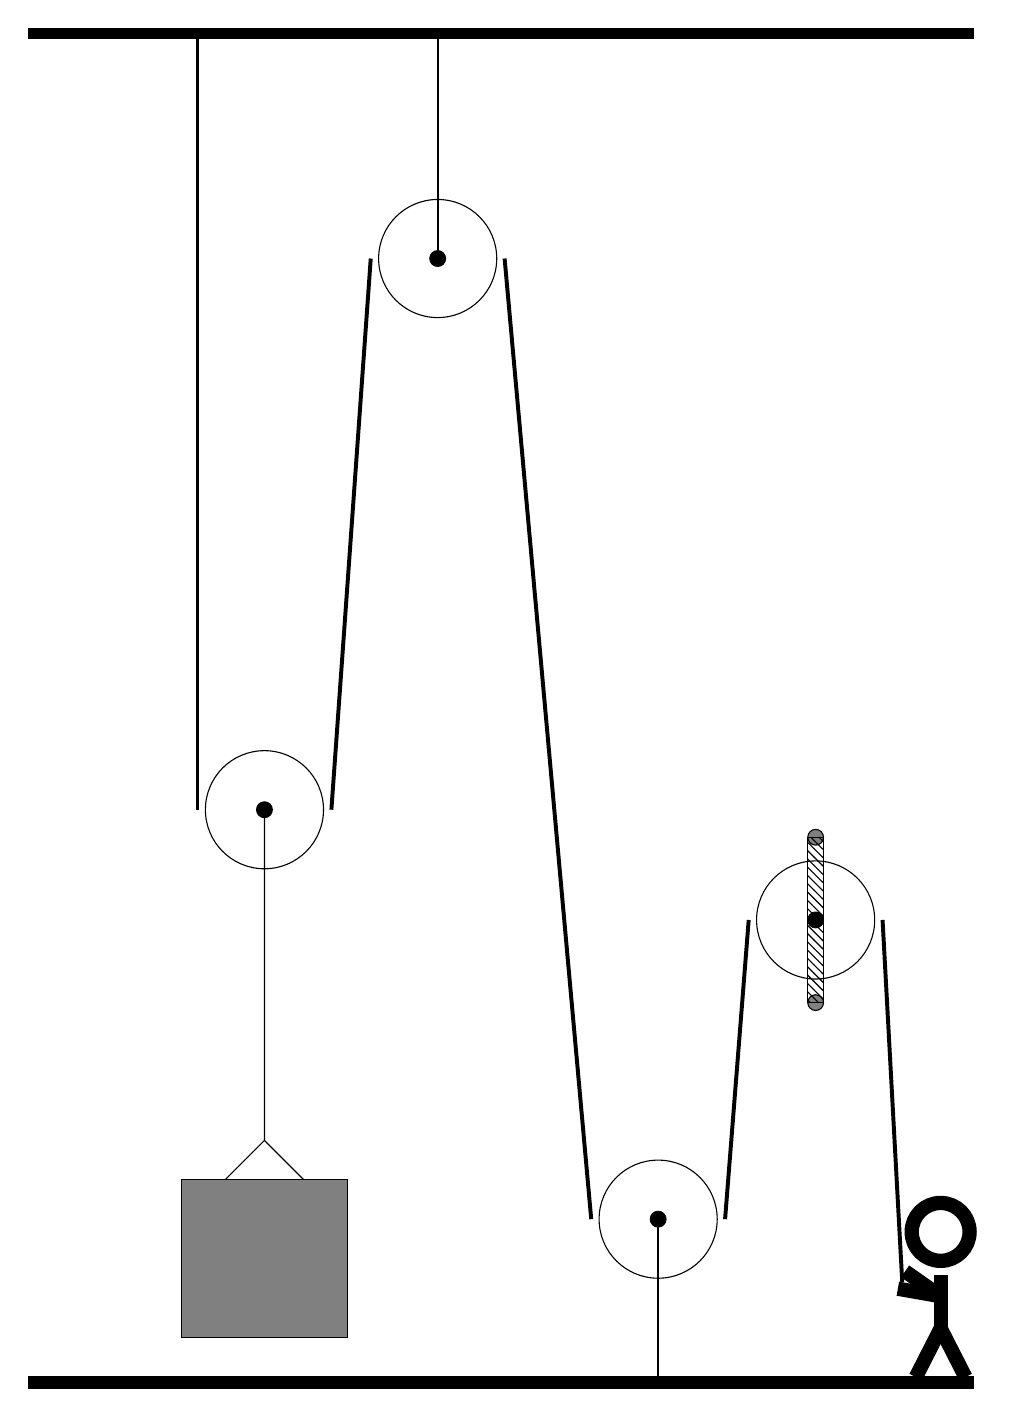
\begin{tikzpicture}
		%%%%% START %%%%%
		\draw[fill=black] (-2, 14) rectangle (10, 14.125);
		
		\draw (1, 4.2) circle (0.75);
		\draw[fill=black] (1, 4.2) circle (0.1);
		
		\draw (3.2, 11.2) circle (0.75);
		\draw[fill=black] (3.2, 11.2) circle (0.1);
		\draw[thick] (3.2, 11.2) -- (3.2, 14);
		
		\draw (6, -1) circle (0.75);
		\draw[fill=black] (6, -1) circle (0.1);
		\draw[thick] (6, -1) -- (6, -3);
		
		\draw[fill=white](8, 2.8) circle (0.75);
		\draw[fill=black] (8, 2.8) circle (0.1);
		\draw[fill=black!50] (8, 3.85) circle (0.1);
		\draw[fill=black!50] (8, 1.75) circle (0.1);
		\draw[pattern=north west lines, pattern color=black] (7.9, 3.85) rectangle (8.1, 1.75);
		
		\draw (1, 4.2) -- (1, 0) -- (0.5, -0.5);
		\draw (1, 0) -- (1.5, -0.5);
		\draw[fill=black!50] (-0.05, -0.5) rectangle (2.05, -2.5);
		
		\draw[line width=0.5mm] (0.15, 14) -- (0.15, 4.2);
		\centerarc[line width=0.5mm](1, 4.2)(180:360:0.85);
		\draw[line width=0.5mm](1.85, 4.2) -- (2.35, 11.2);
		\centerarc[line width=0.5mm](3.2, 11.2)(0:180:0.85);
		\draw[line width=0.5mm](4.05, 11.2) -- (5.15, -1);
		\centerarc[line width=0.5mm](6, -1)(180:360:0.85);
		\draw[line width=0.5mm](6.85, -1) -- (7.15, 2.8);
		\centerarc[line width=0.5mm](8, 2.8)(0:180:0.85);
		\draw[line width=0.5mm](8.85, 2.8) -- (9.1, -1.8);
		
		\node at (9.5, -1.9) {\Strichmaxerl[10][-35][170]};
		
		\draw[fill=black] (-2, -3) rectangle (10, -3.15);
		%%%%% END %%%%%
	\end{tikzpicture}
\end{document}